\chapter{Experiments \& Results}\label{chap:results}

  \section{ELA-DenseNet} \label{sec:s1}

In this section, we delve into the experimental journey of the proposed classification model before deciding on the DenseNet-121 architecture as the preferred CNN backbone making up the final ELA-DenseNet model. These preliminary experiments explore various architectures, methodologies, and fine-tuning strategies, providing insights into the model's evolution and guiding the ultimate selection of DenseNet-121. This section presents a retrospective analysis of the experimental iterations, paving the way for a comprehensive understanding of the model's development and the rationale behind its architectural choices.

Initially, the first models implemented were simple sequential CNNs trained from scratch without leveraging any pre-trained weights. These models, as with all subsequent models, were trained on the CASIA V2 dataset. These `primitive' models generalized very poorly despite configurations to reduce overfitting. This behavior was the motivation for a shift towards transfer learning and adopting pre-trained models as backbone architectures. 

After extensive research, the CNN-backbone candidates were chosen, namely: AlexNet, DenseNet-121, Xception and VGG16. They were chosen based on their proven ability to perform well on image classification tasks \cite{MeenaTyagi2019}. All of the models were used in conjunction with the ELA component. Training time was an important factor in the selection process given limited computational resources and the time-constrained nature of the project. All models had the pre-trained ImageNet weights loaded and were set to train for 30 epoch with an RMSprop optimizer and an early stopping mechanism as described in the Proposed Model section above. Notably, the Xception model took almost 4x as much training time as the DenseNet-121 model despite an expected similar training time due to their relatively similar architecture complexity. 

The metrics used to evaluate the models included accuracy, recall, and F1-score. Accuracy, a basic measure reflecting overall correctness, is calculated by dividing correct predictions (true positives and true negatives) by the total number of predictions. Precision and recall, key components of the F1-score, assess positive prediction accuracy and the model's ability to capture all positive instances, respectively. The F1 score combines these metrics into a single value, providing a comprehensive assessment of model performance on a scale from 0 to 1. A higher F1 score indicates a better balance between precision and recall. Comparative results for candidate models are presented in Table \ref{table:Candidates}. The DenseNet model outperformed others, achieving 93.2\% accuracy and an F1-Score of 0.881 with a 0.959 recall on the CASIA V2 dataset.

In the realm of image forgery detection, especially in combating misinformation, achieving good recall is paramount. Recall measures the model's effectiveness in identifying all instances of forged images, reducing the risk of misinformation going undetected. High recall, prioritized to capture as many instances of image forgery as possible, helps minimize false negatives and ensures a comprehensive identification of deceptive content. While this emphasis on recall may come at the expense of precision, the overarching objective is to reduce instances of misinformation evading detection. In the battle against misinformation, a robust recall is fundamental for fostering public trust and upholding the integrity of information channels, contributing to a more reliable and secure digital landscape.


\begin{align*}
\text{Accuracy} & = \frac{TP + TN}{TP + TN + FP + FN} \\
\text{Precision} & = \frac{TP}{TP + FP} \\
\text{Recall} & = \frac{TP}{TP + FN} \\
\text{F1 Score} & = \frac{2 \times \text{Precision} \times \text{Recall}}{\text{Precision} + \text{Recall}} = \frac{2 \times TP}{2 \times TP + FP + FN}
\end{align*}

\begin{table}[!h]
\centering
\begin{tabular}{|l|c|c|c|c|}
\hline
Base Model & Accuracy & Precision & Recall & F1-Score \\
\hline
AlexNet & 0.831 & 0.850 & 0.767 & 0.806 \\ \hline
VGG16 & 0.887 & 0.802 & 0.758 & 0.778 \\ \hline
Xception & 0.907 & \textbf{0.874} & 0.876 & 0.875 \\ \hline
DenseNet-121 & \textbf{0.932} & 0.856 & \textbf{0.959} & \textbf{0.901} \\ \hline
\end{tabular}
\caption{Comparisons of the candidate models on CASIA V2}
\label{table:Candidates}
\end{table}


To benchmark against existing ELA-based splicing detection models such as \cite{zhang2021image} and the original ELA model outlined in \cite{krawetz2007picture}, our proposed ELA-DenseNet underwent evaluation using the Columbia dataset. Additionally, the state-of-the-art MiniNet deep learning model \cite{tyagi2023mininet}, chosen for its absence of an ELA component, required manual testing on the Columbia dataset due to its initially reported results being based on experiments with the CASIA V2 dataset. The results in Table \ref{table:benchmarks} indicate that ELA-DenseNet surpasses these benchmarks, achieving an accuracy of 95.1\% and an F1-Score of 0.936 with emphasis on a higher recall.

\begin{table}[!h]
\centering
\begin{tabular}{|l|c|c|c|c|}
\hline
Model & Accuracy & Precision & Recall & F1-Score \\ \hline
ELA  & 0.223 &  0.796 & 0.113& 0.237 \\ \hline
ELA-LBP & 0.914 & 0.901 & 0.932 & 0.917 \\ \hline
MiniNet & 0.867 & 0.852 & 0.791 & 0.819 \\ \hline
ELA-DenseNet & \textbf{0.951} & \textbf{0.913} & \textbf{0.966} & \textbf{0.936} \\ \hline
\end{tabular}
\caption{Comparisons of the proposed model against benchmarks on the Columbia dataset}
\end{table}
\label{table:benchmarks}


  \section{Fine-tuned Vision Transformer} \label{sec:s2}
  
The performance of the ViT-IML model is thoroughly examined by training it on the InTheWild \cite{huh2018fighting} dataset, revealing an initially suboptimal performance of the original model as shown under the `OG Predict' and `After thresholding' masks. Finetuning the model involved initially employing the Adam optimizer, as shown in Figure \ref{fig:ViTAdam}, and subsequently transitioning to the Stochastic Gradient Descent (SGD) optimizer, as shown in Figure \ref{fig:ViTSGD}.

To ensure a fair and meaningful comparison, the performance of the models was tested on the CASIA V1 dataset and the Columbia dataset - the same datasets used to derive the published results for the original ViT-IML model. The metrics used for evaluation are pixel-level F1 score with a fixed threshold 0.5 and pixel-level Area Under Curve (AUC), which are commonly used metrics in previous works. In some evaluation methods, determining the optimal threshold for the F1 score can be challenging due to variations in real-world data distributions. To address this, the pixel-level F1 score is proposed as an alternative metric, using a fixed threshold of 0.5. This approach offers a practical and interpretable measure for assessing a model's performance at the pixel level, making it more suitable in scenarios where finding an optimal threshold is uncertain or impractical. The use of a consistent threshold enhances the applicability and reliability of the evaluation process, especially in real-world, dynamic environments. This evaluation and its metrics aim to determine the overall impact of fine-tuning on the new model's ability to generalize when compared directly with its predecessor. By conducting these tests on the familiar ground of the CASIA V1 and Columbia datasets, we establish a consistent benchmark to validate improvements and ascertain the model's efficacy in real-world scenarios.

The results of the tests are shown in Table \ref{table:vitresults}. The comparative analysis demonstrates that the SGD optimizer yields superior results. The table also shows the results of finetuning on the ExpandedInTheWild dataset, more than double the size of the InTheWild. As expected, the model's performance improved with enriched data with an F1 score of 0.721  and AUC of 0.915 on the CASIA V1 dataset compared to an F1 score of 0.704 an AUC of 0.892 from fine-tuning on the smaller dataset.



\begin{figure}
    \centering
    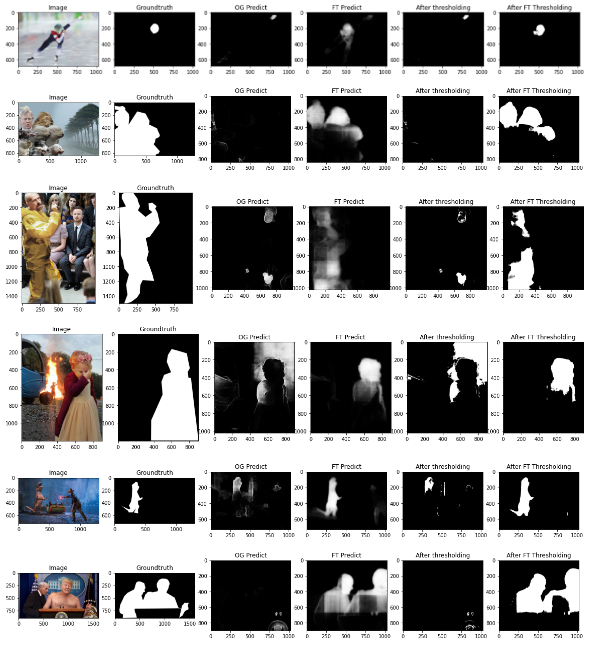
\includegraphics[width=0.9\linewidth]{ViTAdam.png}
    \caption{Comparison of before and after fine-tuning (FT) with Adam}
    \label{fig:ViTAdam}
\end{figure}

\begin{figure}
    \centering
    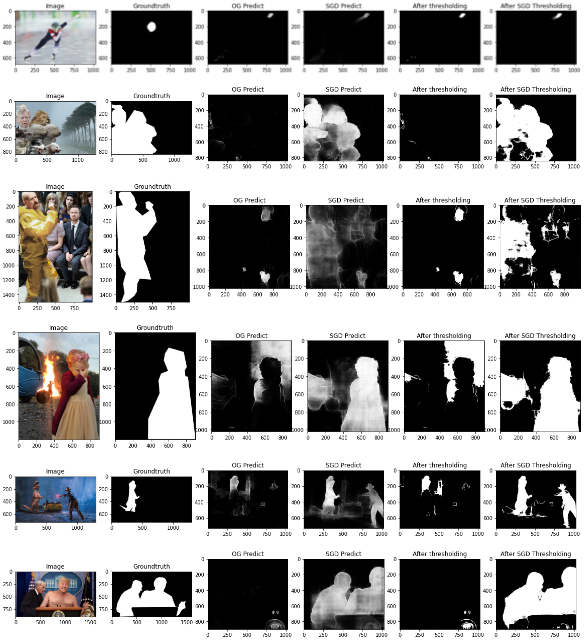
\includegraphics[width=1\linewidth]{ViTSGD.png}
    \caption{Comparison of before and after fine-tuning with SGD}
    \label{fig:ViTSGD}
\end{figure}

\begin{table}[]
\centering
\small
\begin{tabular}{|l|ll|ll|}
\hline
\multicolumn{1}{|c|}{\multirow{2}{*}{Model}} & \multicolumn{2}{c|}{CASIA V1} & \multicolumn{2}{c|}{Columbia} \\ \cline{2-5} 
\multicolumn{1}{|c|}{} & \multicolumn{1}{c|}{PL F1} & \multicolumn{1}{c|}{PL AUC} & \multicolumn{1}{c|}{PL F1} & \multicolumn{1}{c|}{PL AUC} \\ \hline
\textit{ViT-IML} & \multicolumn{1}{l|}{\textit{0.658}} & \textit{0.867} & \multicolumn{1}{l|}{\textit{0.836}} & \textit{0.908} \\ \hline
Adam-ViT-IML & \multicolumn{1}{l|}{0.673} & 0.874 & \multicolumn{1}{l|}{0.842} & 0.912 \\ \hline
SGD-ViT-IML & \multicolumn{1}{l|}{\textbf{0.704}} & \textbf{0.892} & \multicolumn{1}{l|}{\textbf{0.864}} & \textbf{0.922} \\ \hline
SGD-ViT-IML (Expanded) & \multicolumn{1}{l|}{\textbf{\textit{0.721}}} & \textbf{\textit{0.915}} & \multicolumn{1}{l|}{\textbf{\textit{0.887}}} & \textbf{\textit{0.931}} \\ \hline

\end{tabular}
\caption{Results of the fine-tuned models on test datasets. The bolded italics show the results after fine-tuning on the ExpandedInTheWild dataset.}
\end{table}
\label{table:vitresults}